\documentclass{ieeeaccess}
%Adjusted 05/13/2026 at the byline author names
\usepackage{cite}
\usepackage{amsmath,amssymb,amsfonts}
\usepackage{algorithmic}
\usepackage{algorithm}
\usepackage{graphicx}
\usepackage{textcomp}
\usepackage{caption}
\usepackage{subcaption}
%\usepackage{algpseudocode}
\usepackage{enumerate}
\usepackage{siunitx}

\usepackage{bm}
\makeatletter
\AtBeginDocument{\DeclareMathVersion{bold}
\SetSymbolFont{operators}{bold}{T1}{times}{b}{n}
\SetSymbolFont{NewLetters}{bold}{T1}{times}{b}{it}
\SetMathAlphabet{\mathrm}{bold}{T1}{times}{b}{n}
\SetMathAlphabet{\mathit}{bold}{T1}{times}{b}{it}
\SetMathAlphabet{\mathbf}{bold}{T1}{times}{b}{n}
\SetMathAlphabet{\mathtt}{bold}{OT1}{pcr}{b}{n}
\SetSymbolFont{symbols}{bold}{OMS}{cmsy}{b}{n}
\renewcommand\boldmath{\@nomath\boldmath\mathversion{bold}}}
\makeatother

\def\BibTeX{{\rm B\kern-.05em{\sc i\kern-.025em b}\kern-.08em
    T\kern-.1667em\lower.7ex\hbox{E}\kern-.125emX}}

%Your document starts from here ___________________________________________________
\begin{document}
\history{Date of publication xxxx 00, 0000, date of current version xxxx 00, 0000.}
\doi{10.1109/ACCESS.2024.0429000}

\title{Preparation of Papers for IEEE ACCESS}
\author{\uppercase{First A. Author}\authorrefmark{1}, \IEEEmembership{Fellow, IEEE},
\uppercase{Second B. Author}\authorrefmark{2}, AND \uppercase{Third C. Author},
Jr.\authorrefmark{3},
\IEEEmembership{Member, IEEE}}

\address[1]{National Institute of Standards and
Technology, Boulder, CO 80305 USA (e-mail: author@boulder.nist.gov)}
\address[2]{Department of Physics, Colorado State University, Fort Collins,
CO 80523 USA (e-mail: author@lamar.colostate.edu)}
\address[3]{Electrical Engineering Department, University of Colorado, Boulder, CO
80309 USA}
\tfootnote{This paragraph of the first footnote will contain support
information, including sponsor and financial support acknowledgment. For
example, ``This work was supported in part by the U.S. Department of
Commerce under Grant BS123456.''}

\markboth
{Author \headeretal: Preparation of Papers for IEEE TRANSACTIONS and JOURNALS}
{Author \headeretal: Preparation of Papers for IEEE TRANSACTIONS and JOURNALS}

\corresp{Corresponding author: First A. Author (e-mail: author@ boulder.nist.gov).}


\begin{abstract}
Current development of microservice architectures heavily relies on API gateways and high-performance RPC frameworks like gRPC, the implementation details of the inter-service communication layer are often abstracted away in system design. Our paper empirically investigates the performance degradation caused by application-layer communication bottlenecks, with particular focus on gRPC connection management. We present a mathematical queueing model and algorithmic formalization to quantify the overhead of the connection-per-request (CPR) compared to a persistent channel reuse (PCR). Our evaluation results in Kubernetes environment tests show that converting CPR to PCR models can significantly reduce median latency by 97\%—from over 7,000 ms to 150 ms under peak load. This change significantly eliminates the performance bottleneck that caused an increase in end-to-end user experience latency time.
\end{abstract}

\begin{keywords}
Cloud-Native, Connection Per Request, gRPC API, High Performance Computing, Kubernetes, Microservices, Persistent Channel Reuse 
\end{keywords}

\titlepgskip=-21pt

\maketitle

%%%%%%%%%%%%%%%%%%%%%%%%%%%%%%%%%%%%%%%%%%%%%%%%
\section{Introduction}
\label{sec:introduction}
%%%%%%%%%%%%%%%%%%%%%%%%%%%%%%%%%%%%%%%%%%%%%%%%

\PARstart{T}{he} transition to cloud-native microservices has established API gateways and high-performance RPC frameworks like gRPC as standard infrastructure. In this architecture, the API gateway functions as the singular entry point for external traffic, acting primarily as a reverse proxy and protocol transcoder. While external clients typically communicate using standard HTTP/1.1 and JSON payloads—often following RESTful paradigms as discussed in \cite{martin2022online}—internal microservices increasingly rely on gRPC over HTTP/2 for high-performance communication \cite{Ventre2018SDNAAA}. Unlike the stateless nature of traditional REST, gRPC is specifically designed to multiplex many requests over a single persistent HTTP/2 connection. However, the implementation details of this inter-service communication layer are often abstracted away by frameworks. As study by \cite{zhu2023dissecting}, have exposed significant infrastructural overheads hidden within service mesh sidecars, we observe that analogous, undocumented performance penalties exist within the application layer of API gateways when protocol translations are mismanaged.

The specific issue addressed in this paper is the performance degradation caused by the "connection-per-request" (CPR) anti-pattern within these gateways. Previous studies have shown how TCP and TLS handshake delays reduce throughput in distributed systems \cite{Guo2020StatefulTCPANAA}. However, the direct application of legacy REST-based connection management to gRPC environments remains a pervasive flaw. We define gRPC connection churn as the continuous cycle of establishing and tearing down complex network state (TCP handshakes and HTTP/2 protocol negotiations) for every individual application-layer request, rather than multiplexing traffic. Establishing a new connection per request is an $O(N)$ operation, where $N$ represents the number of incoming client requests. This directly conflicts with the $O(1)$ multiplexed design of HTTP/2, forcing gateway worker threads to spend excessive CPU cycles on network context switching. We explore this vulnerability using a standard Python WSGI stack \cite{wsgi-pep} (Flask and Gunicorn) as a representative testbed, as its synchronous worker model clearly exposes the severe latency penalties of blocking network I/O.

While the research community has modeled microservice performance extensively, the specific intersection of application-layer connection churn and queueing network saturation remains empirically unquantified. Recent academic works, such as those by Pinheiro et al. \cite{pinheiro2024performance}, utilize stochastic Petri Nets to evaluate microservice resilience; however, evaluating latency under load requires a shift toward queueing theory. We argue that bottlenecks at the implementation level, particularly the phenomenon of gRPC connection churn, lead to a dynamic increase in the service time ($S$) of the system. In queueing theory \cite{DAuria2021AnMQA}, an inflated service time severely degrades the theoretical service rate ($\mu$). This churn converts what should be a constant-time RPC execution into a highly variable, load-dependent event. Previous research has not addressed how this specific application-layer mismanagement forces premature queue saturation long before physical CPU or memory limits are reached.

Therefore, this paper demonstrates how converting the original CPR approach into a Persistent Channel Reuse (PCR) approach, as shown in the Fig. \ref{fig1}—by refactoring the gateway code to initialize a global, thread-safe gRPC channel at startup—eliminates this bottleneck. To validate this, the specific contributions of this paper are as follows:

\begin{itemize}
    \item We model the request patterns and application-layer logic based on both the CPR and the refactored PCR approaches.
    
    \item We introduce a queueing-theoretic model to explain the non-linear latency spikes observed under high load, linking application-layer connection churn to queue saturation.
    
    \item We benchmark these models within an actual Kubernetes environment using controlled isolation environment—\break{ensuring} the gateway is evaluated independently of backend database or business logic variance—to validate the correctness of the theoretical model against empirical runs.
\end{itemize}

%\begin{figure}
%  \centering
%  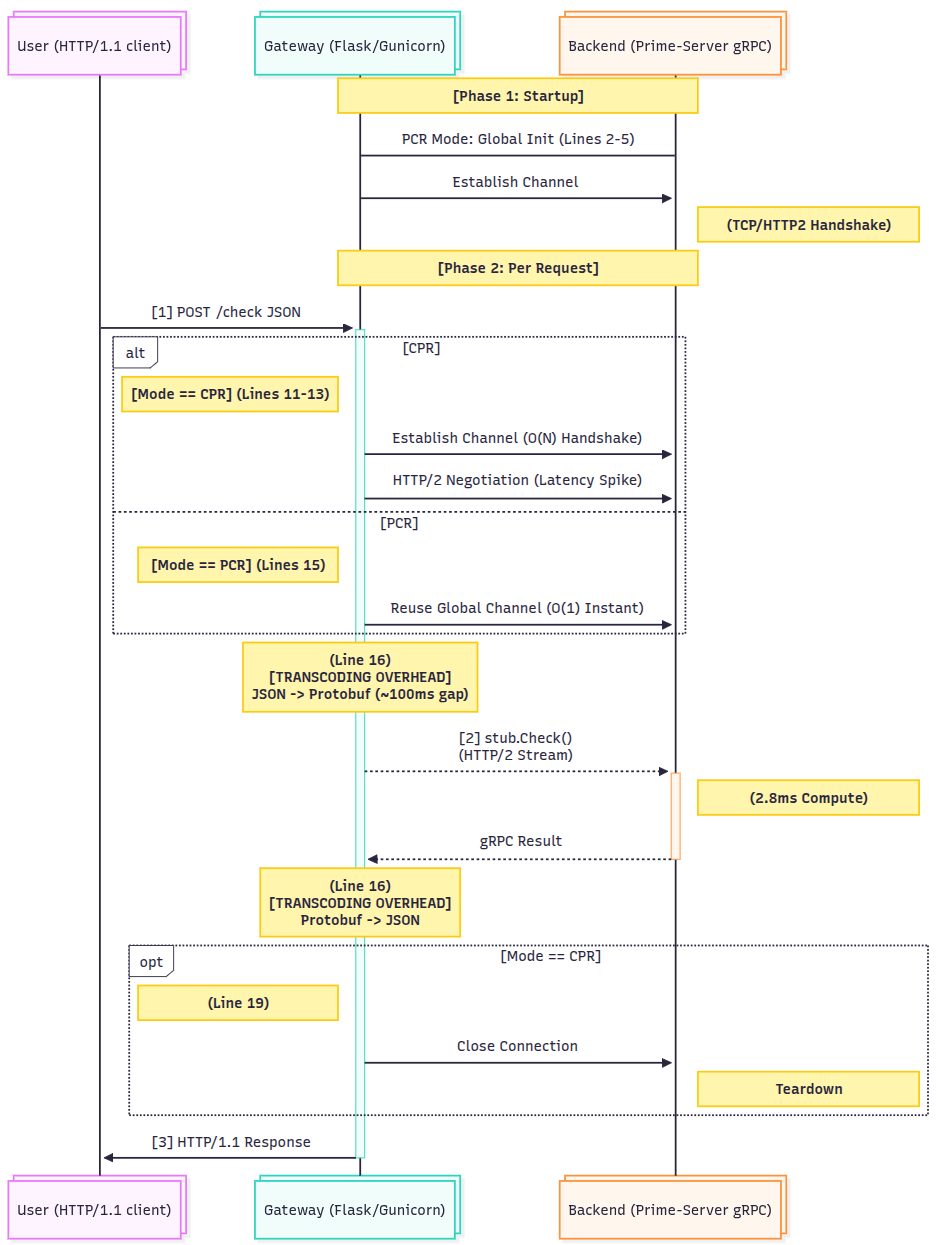
\includegraphics[width=\columnwidth,height=0.6\textheight,keepaspectratio]{fig/PCRvsCPR-SeqDiagram.png} % or \linewidth
%  \caption{The framework models of gRPC connections mechanism. Connection-Per-Request (CPR) vs Persistent Connection Reuse (PCR).}
%  \label{fig1}
%\end{figure}

\begin{figure*}[t]
	\centering
	\begin{subfigure}[t]{0.47\textwidth}
		\centering
		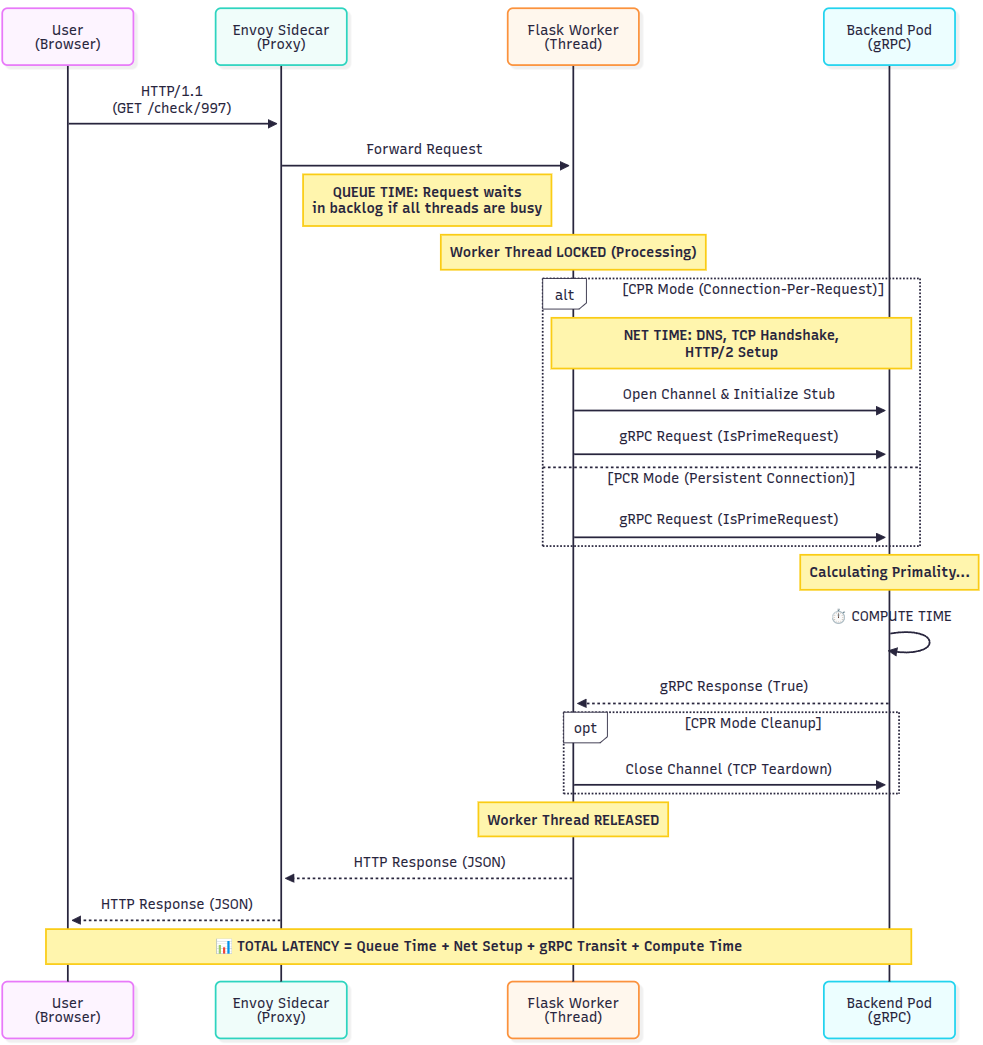
\includegraphics[width=\linewidth]{fig/seq-diagram-1-sync.png}
		\caption{Synchronous CPR/PCR (Flask/Gunicorn).}
		\label{fig:seq1}
	\end{subfigure}
	\hfill
	\begin{subfigure}[t]{0.47\textwidth}
		\centering
		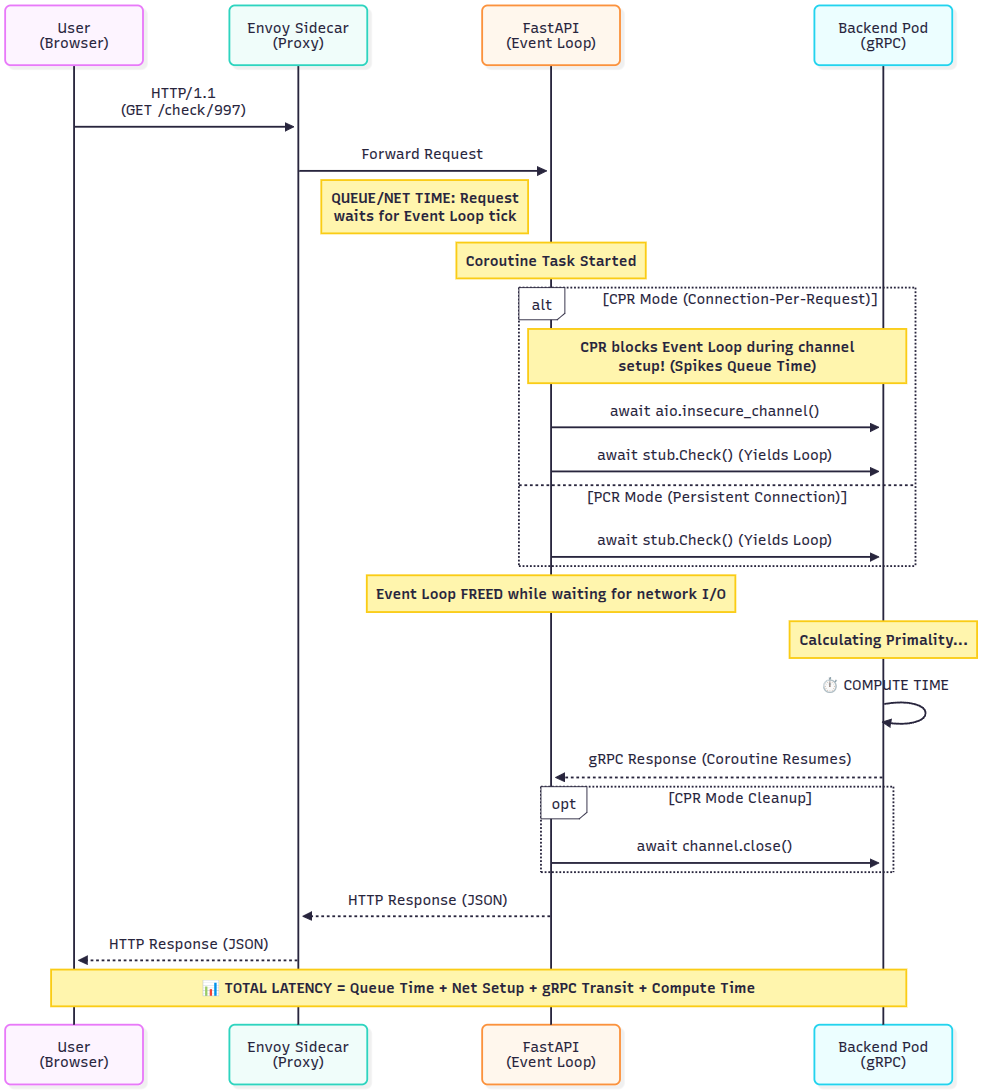
\includegraphics[width=\linewidth]{fig/seq-diagram-2-async.png}
		\caption{Asynchronous CPR/PCR (Flask/Uvicorn).}
		\label{fig:seq2}
	\end{subfigure}
	\caption{Sequence process of synchronous vs asynchronous communication models of cloud-native application.}
	\label{fig:seq-model}
\end{figure*}

%%%%%%%%%%%%%%%%%%%%%%%%%%%%%%%%%%%%%%%%%%%%%%%%
\section{Mathematical Modeling of gRPC Connection Management}
\label{sec2}
%%%%%%%%%%%%%%%%%%%%%%%%%%%%%%%%%%%%%%%%%%%%%%%%

In order to comprehend the communication bottleneck, it is essential to break down the entire lifecycle of a request as it progresses through the API gateway. This analysis will help us identify the key stages and factors contributing to the bottleneck in the communication process.

Let $T_{total}$ be the total end-to-end latency experienced by the client. We define $T_{total}$ as:
\begin{equation}
    T_{\text{total}} = T_{\text{http}} + W_{\text{queue}} + S_{\text{gateway}} + T_{\text{network}}
\end{equation}

Where:
\begin{description}
  \item[$T_{\text{http}}$]    : ingress HTTP processing time.
  \item[$W_{\text{queue}}$]   : queueing delay at the gateway's worker processes.
  \item[$S_{\text{gateway}}$] : service time required by the gateway to establish and execute the downstream gRPC call.
  \item[$T_{\text{network}}$] : physical network propagation delay and backend computation time (baseline constant $c \approx 3\ \text{ms}$).
\end{description}

The critical variable in our study is $S_{gateway}$. We model this under two distinct operational paradigms.

\subsection{Paradigm 1: Connection-Per-Request (CPR)}
\label{sec2.1}

In the CPR anti-pattern, as shown in the Fig. \ref{fig:seq-model} at the CPR sections, the gateway initializes a new gRPC channel for every incoming request. The service time $S_{cpr}$ is defined as:

\begin{equation}
    S_{cpr} = t_{tcp} + t_{http2} + t_{rpc} + t_{teardown}
\end{equation}

Where $t_{tcp}$ is the TCP 3-way handshake, $t_{http2}$ is the HTTP/2 SETTINGS frame negotiation, $t_{rpc}$ is the actual payload serialization/transmission, and $t_{teardown}$ is the TCP teardown (FIN/ACK). Because $t_{tcp}$ and $t_{http2}$ require multiple network round-trip times (RTTs) and significant CPU context switching, $S_{cpr} \gg t_{rpc}$.

In decentralized cloud-native architectures, the Client-side Proxy Routing (CPR) model dictates that the primary application container natively executes its own network routing and load balancing (e.g., utilizing native gRPC load balancing). This proxyless architecture minimizes intermediate network hops, optimizing baseline latency and reducing steady-state resource consumption. However, previous studies on proxyless service meshes demonstrate a critical vulnerability: the CPR model tightly couples the computational domain with the networking domain.

From a queueing theory perspective, the CPR model operates as a rigid $M/M/c$ queue. Under acute traffic surges, the network routing logic aggressively competes with the core application logic for limited CPU cycles and thread pools. When the system arrival rate approaches or exceeds the mathematical processing capacity ($\lambda \ge  \lambda_{sat}$), the application’s internal queue saturates rapidly, inevitably leading to dropped connections, unbounded tail latency, and catastrophic node failure.

\subsection{Paradigm 2: Persistent Channel Reuse (PCR)}
\label{sec2.2}

In the optimized PCR pattern, as shown in Fig. \ref{fig:seq-model} at PCR sections, the gateway initializes a single, thread-safe gRPC channel during application startup. All incoming requests are multiplexed over this channel. The setup costs are amortized over millions of requests, approaching zero per request. Thus, the service time $S_{pcr}$ simplifies to:

\begin{equation}
    S_{pcr} = t_{rpc}
\end{equation}

Conversely, the PCR model completely decouples the data plane from the application by offloading routing, load balancing, and telemetry to a dedicated, out-of-process sidecar proxy (such as Envoy).

While conventional research often criticizes the PCR model for introducing a continuous ``service mesh tax''—permanent CPU, memory, and latency overheads during normal operations—its architectural strength lies in robust queue management. In the PCR model, the sidecar acts as a highly optimized, asynchronous buffer. It is capable of absorbing massive traffic spikes, managing connection backlogs, and applying intelligent backpressure, thereby protecting the underlying application container from localized saturation.

\subsection{Queueing Theory and Non-Linear Saturation}
\label{sec2.3}

The catastrophic latency spikes observed in empirical testing (e.g., jumping to 7,000 ms) cannot be explained by $S_{cpr}$ alone. We must apply an $M/M/c$ queueing model, where incoming requests arrive at rate $\lambda$ and are serviced by $c$ gateway worker threads at rate $\mu = 1/S_{gateway}$.

The utilization of the gateway system is $\rho = \frac{\lambda}{c \cdot \mu}$.
According to Little's Law \cite{little2011or} and standard queueing theory, the average queueing delay $W_{queue}$ grows asymptotically as utilization $\rho \to 1$:

\begin{equation}
    W_{queue} \propto \frac{\rho}{1 - \rho}
\end{equation}

Because $S_{cpr}$ is significantly larger than $S_{pcr}$, the service rate $\mu_{cpr}$ is artificially low. Therefore, under the CPR paradigm, the system reaches critical utilization ($\rho \to 1$) at a much lower arrival rate $\lambda$ (e.g., 400 RPS). When $\lambda$ exceeds this threshold (e.g., 600 RPS), $W_{queue}$ approaches infinity, resulting in the massive latency spikes and connection timeouts observed in our baseline data.

To fully contextualize the performance disparity between these (CPR and PCR) approaches, it is necessary to distinguish the roles of the TCP session, the HTTP/2 stream, and the application-layer channel management. A \textbf{TCP session} represents the underlying Layer-4 network socket, which incurs significant latency overhead to establish (e.g., 3-way handshakes). An \textbf{HTTP/2 stream} is a lightweight, logical sequence of frames operating within that single TCP session; this is the native mechanism gRPC uses to multiplex thousands of concurrent requests over one connection. 

The essential flaw of the CPR anti-pattern is that it actively circumvents this multiplexing capability. By instantiating and tearing down a gRPC channel within the local request handler, CPR forces the underlying HTTP/2 library to establish and destroy a unique TCP session for every single request, effectively limiting multiplexing to a single stream per connection. Conversely, the Persistent Channel Reuse (PCR) approach does not rebuild HTTP/2 features in the application layer; rather, it is a structural design pattern that initializes a single, global TCP session at startup. This application-layer refactoring is strictly an enabler, keeping the L4 connection persistent so that the native L7 HTTP/2 stream multiplexing can function as originally intended.

\subsection{Proactive Autonomic Controller via $M/M/c$ Queueing}
\label{sec2.4}

To mathematically formalize the system's performance under increasing target rates, the system architecture can be modeled as an $M/M/c$ queue. This assumes a Poisson arrival process for incoming requests with rate $\lambda$ (target rate), exponentially distributed service times with rate $\mu$ (where $\mu = 1 / T_{compute}$), and $c$ parallel computing resources \cite{tijms2003first} \cite{Banerjee2023MTDDHJSMTA}.

For the system to remain stable, $\rho < 1$. As the target rate $\lambda$ increases toward the total service capacity $c\mu$, the system enters a state of high utilization. According to Erlang's C formula, the probability that an arriving request must wait in the queue ($P_Q$) is:

\begin{equation}
	P_Q = \frac{\frac{(c\rho)^c}{c!(1-\rho)}}{\sum_{n=0}^{c-1} \frac{(c\rho)^n}{n!} + \frac{(c\rho)^c}{c!(1-\rho)}}
\end{equation}

Consequently, the average expected wait time in the queue ($W_q$) grows non-linearly $$W_{queue} = \frac{P_Q}{c\mu(1-\rho)}$$. As $\rho \to 1$, $W_{queue}$ approaches infinity. This mathematical phenomenon explains the severe spikes observed in the empirical $p99$ tail latencies; minor fluctuations in arrival intervals at high utilization cause disproportionate queuing delays ($T_{net\_and\_queue}$).

\begin{enumerate}
	\item \textbf{The Process: Proactive Autonomic Intervention}
	
	A reactive controller waits for the total end-to-end latency ($W = W_q + \frac{1}{\mu}$) to breach a Service Level Agreement (SLA) before intervening. In contrast, the implemented proactive autonomic controller leverages this queueing theory framework to anticipate degradation. Instead of monitoring absolute latency thresholds, the proactive controller monitors the rate of change of the queueing delay with respect to the incoming load ($\frac{\partial W_q}{\partial \lambda}$), or establishes a critical utilization threshold ($\rho_{crit} < 1$).The trigger condition is mathematically defined to activate when the predicted waiting time approaches the upper bound of the acceptable SLA variance:
	

	$$Trigger \rightarrow True \quad \text{if} \quad \rho \ge \rho_{crit} \quad$$ 
	$$\text{or} \quad W_q(\lambda_{t+1}) > SLA_{threshold}$$

	
	Upon triggering, the autonomic mechanism intervenes proactively—typically by scaling the number of resources ($c \to c'$) or applying backpressure to throttle incoming requests ($\lambda \to \lambda'$). By dynamically increasing the denominator ($c'\mu$) or capping the numerator ($\lambda'$), the controller artificially forces $\rho$ back to a stable state ($\rho < \rho_{crit}$), effectively neutralizing the exponential queuing delay before the physical system exhibits SLA violations.
	
	\item \textbf{Mitigation of Connection Bottlenecks via the PCR Autonomic Controller}
	
	In traditional Connection Per Request (CPR) architectures, $T_{net\_and\_queue\_ms}$ serves as the primary indicator of connection bottlenecks, as exhausted connection pools force requests into extended waiting states. Under normal circumstances, this results in a strong positive correlation between load ($\lambda$) and queueing delay ($W_{queue}$). However, our empirical analysis of the implemented PCR (Connection/Compute-to-Queue) model demonstrates a disruption of this bottleneck paradigm. A Pearson correlation analysis revealed a surprisingly weak and statistically insignificant relationship between target rate and queue time ($r = 0.1410, p = 0.059$). This decoupled relationship indicates that the system does not succumb to exponential queueing under high concurrency.The mechanism behind this stability is the highly proactive autonomic controller. A point-biserial correlation confirmed a strong, highly significant relationship between the target load and the controller's triggered state ($r_{pb} = 0.8607$, $p < 0.0001$). Furthermore, logistic regression modeling established that the controller is acutely sensitive to early-stage network degradation; for every 1ms increase in queue time, the odds of an autonomic intervention increase by a factor of 1.89. Ultimately, these mathematical findings prove that the PCR model proactively restructures resources at the earliest signs of latency variation, successfully capping the connection bottleneck long before catastrophic CPR-style queuing can occur.
	
\end{enumerate}

%Recent literature predominantly treats CPR and PCR as mutually exclusive, static deployment strategies[cite][cite]. System architects are typically forced to choose between the high-performance, low-overhead proxyless approach (CPR) and the highly resilient, resource-intensive sidecar approach (PCR).

%Existing solutions fail to address the necessity for dynamic architectural elasticity. Static CPR deployments remain fundamentally fragile under catastrophic load, while static PCR deployments waste critical compute resources during periods of low traffic. The autonomic control framework proposed in this paper bridges this gap by introducing a real-time topology transition. By continuously monitoring the $M/M/c$ queue boundaries, the system mathematically predicts failure and mechanically pivots from CPR to PCR only when intervention is strictly required, dynamically balancing steady-state efficiency with transient survivability.

Our current autonomic control framework directly solves the lacked architectural elasticity by bridging the two states dynamically. Rather than waiting for system utilization to fail ($\rho \ge 1.0$), the controller continuously polls real-time telemetry to compute the empirical service time ($S_{cpr}$) and calculates the mathematical saturation limit ($\lambda_{sat}$) based on the application's thread concurrency ($c$):

$$\lambda_{sat} = \frac{c}{S_{cpr}}$$

To guarantee survivability, the controller does not wait for absolute saturation. Instead, it defines a predictive intervention boundary ($\lambda_{trigger}$) using a configurable safety threshold ratio ($T_{ratio}$):

$$\lambda_{trigger} = \lambda_{sat} \times T_{ratio}$$

By continuously monitoring this mathematical boundary, the system can autonomously pivot the Kubernetes architecture from the low-overhead CPR topology to the highly resilient PCR topology in real-time. It executes the Envoy injection exclusively when the incoming traffic ($\lambda$) breaches the predictive trigger ($\lambda \ge \lambda_{trigger}$), successfully balancing steady-state efficiency with transient survivability.

%%%%%%%%%%%%%%%%%%%%%%%%%%%%%%%%%%%%%%%%%%%%%%%%%%%%%%%%%%%%%%%%%%%%%%%
\section{Algorithmic Formalization}
\label{sec3}
%%%%%%%%%%%%%%%%%%%%%%%%%%%%%%%%%%%%%%%%%%%%%%%%%%%%%%%%%%%%%%%%%%%%%%%

The primary objective of Algorithm~\ref{alg1} is to map the abstract queueing variables from Section \ref{sec2} directly to their application-layer implementations. It illustrates exactly where gateway service time ($S_{gateway}$) is consumed by contrasting both configurations.

Under the Connection-Per-Request (CPR) paradigm, channel initialization and teardown occur locally within the request handler (Lines 10-12, 17-19). This imposes an $O(N)$ computational penalty, manifesting as the "connection churn" that degrades the service rate ($\mu$). Conversely, the Persistent Channel Reuse (PCR) paradigm shifts this network state management to a global, one-time execution at startup (Lines 2-5). By referencing a thread-safe, multiplexed channel ($O(1)$ overhead), the structural refactoring averts queue saturation without altering the core RPC business logic.

\begin{algorithm}
\caption{API Gateway Request Handler: CPR vs. PCR Paradigm}
\label{alg1}
\begin{algorithmic}[1]
\REQUIRE $req\_number$: Integer, $mode$: \{CPR, PCR\}
\ENSURE $is\_prime\_result$: Boolean
\vspace{1mm}
\STATE \textit{// PCR Global Initialization (Executed Once at Startup, $O(1)$)}
\IF{$mode == \text{PCR}$}
    \STATE $global\_channel \gets \text{grpc.insecure\_channel}(\text{SERVER\_ADDRESS})$
    \STATE $global\_stub \gets \text{PrimeCheckerStub}(global\_channel)$
\ENDIF
\vspace{2mm}
\STATE \textbf{function} HandleRequest($req\_number$, $mode$)
    \IF{$mode == \text{CPR}$}
        \STATE \textit{// CPR Local Initialization (Executed per request, $O(N)$)}
        \STATE $channel \gets \text{grpc.insecure\_channel}(\text{SERVER\_ADDRESS})$
        \STATE $stub \gets \text{PrimeCheckerStub}(channel)$
    \ELSE
        \STATE $stub \gets global\_stub$ \textit{// $O(1)$ Memory Reference}
    \ENDIF
    \vspace{1mm}
    \STATE $payload \gets \text{IsPrimeRequest}(\text{number}=req\_number)$
    \STATE $response \gets stub.\text{Check}(payload)$ \textit{// Network I/O}
    \vspace{1mm}
    \IF{$mode == \text{CPR}$}
        \STATE $channel.\text{close}()$ \textit{// Teardown overhead}
    \ENDIF
    \STATE \textbf{return} $response.is\_prime$
\STATE \textbf{end function}
\end{algorithmic}[1]
\end{algorithm}


%\begin{algorithm}
%	\caption{Autonomic Predictive Control for CPR to PCR Transition}
%	\label{alg:autonomic_controller}
%	\begin{algorithmic}[1]
%	\STATE \textbf{Input:} Threshold ratio $T_{ratio}$, Worker threads $c$
%	\STATE \textbf{Output:} Actuation duration $t_{actuation}$ recorded to CSV
%	\STATE \textbf{Function:} \textit{evaluate\_and\_control}
%		\STATE $\lambda \gets \text{QueryMetric}(\text{RPS\_Query})$
%		\STATE $L_{sum} \gets \text{QueryMetric}(\text{Latency\_Sum\_Query})$
%		\IF{$\lambda = 0$}
%		\STATE \textbf{continue} \COMMENT{System stable, no traffic}
%		\ENDIF
%		\STATE $S_{cpr} \gets \frac{L_{sum}}{\lambda}$ \COMMENT{Compute Service Time}
%		\STATE $\lambda_{sat} \gets \frac{c}{S_{cpr}}$ \COMMENT{Calculate Saturation Limit}
%		\STATE $\lambda_{trigger} \gets \lambda_{sat} \times T_{ratio}$ \COMMENT{Calculate Dynamic Threshold}
%			
%		\IF{$\lambda \geq \lambda_{trigger}$}
%		\STATE $t_{start} \gets \text{GetCurrentTime}()$
%		\STATE $\text{PatchDeployment}(\text{EnvoySidecar})$ \COMMENT{Inject Mitigation}
%			
%		\WHILE{$\text{Rollout State} \neq \text{Complete}$}
%		\STATE $\text{Sleep}(2\text{s})$ \COMMENT{Poll API Server}
%		\ENDWHILE
%			
%		\STATE $t_{end} \gets \text{GetCurrentTime}()$
%		\STATE $t_{actuation} \gets t_{end} - t_{start}$ \COMMENT{Measure Actuation Duration}
%%			
%		\STATE \textbf{break} \COMMENT{Idle container for telemetry extraction}
%%			
%		\STATE $\text{Sleep}(5\text{s})$ \COMMENT{Evaluation Interval}
%	\STATE \textbf{End Function}
%	\end{algorithmic}
%\end{algorithm}

\begin{algorithm}
	\caption{Adaptive Autonomic Controller (Phase 2: Dynamic Cutover)}
	\label{alg:autonomic_controller}
	\begin{algorithmic}[1]
		\STATE \textbf{Inputs:} Poll interval $t_{poll}$, Minimum traffic threshold $\lambda_{min} = 10$
		\STATE \textbf{Initialize:} $cutover\_triggered \gets \text{False}$
		\WHILE{\textbf{true}}
		\STATE Sleep for $t_{poll}$ seconds
		\IF{$cutover\_triggered = \text{True}$}
		\STATE \textbf{continue} \COMMENT{Idling post-actuation}
		\ENDIF

		\STATE \COMMENT{Fetch Real-time Telemetry}
		\STATE $\lambda \gets \text{QueryPrometheus}(\text{Rate of Requests (RPS)})$
		\STATE $S_{cpr} \gets \text{QueryPrometheus}(\text{Average Latency (s)})$
		\STATE $n_{threads} \gets \text{QueryPrometheus}(\text{Average Thread Count})$
		
		\IF{$\lambda < \lambda_{min}$ \textbf{or} Telemetry is Null}
		\STATE \textbf{continue} \COMMENT{Wait for stable load}
		\ENDIF

		\STATE \COMMENT{Framework Auto-Detection \& Recalibration}
		\IF{$n_{threads} > 50$}
		\STATE $mode \gets \text{SYNC (Flask)}$
		\STATE $c \gets n_{threads}$ \COMMENT{Capacity bounded by OS threads}
		\STATE $\tau_{ratio} \gets 0.80$
		\ELSE
		\STATE $mode \gets \text{ASYNC (FastAPI)}$
		\STATE $c \gets 3$ \COMMENT{Estimated concurrent event loop tasks}
		\STATE $\tau_{ratio} \gets 0.75$ \COMMENT{Aggressive trigger to prevent starvation}
		\ENDIF

		\STATE \COMMENT{Calculate Saturation Thresholds}
		\STATE $\lambda_{sat} \gets \frac{c}{S_{cpr}}$
		\STATE $\lambda_{trigger} \gets \lambda_{sat} \times \tau_{ratio}$

		\STATE \COMMENT{Evaluate and Actuate}
		\IF{$\lambda \geq \lambda_{trigger}$}
		\STATE $t_{start} \gets \text{CurrentTime}()$
		\STATE $\text{PatchDeployment}(\text{sidecar.istio.io/inject="true"})$
		\STATE $\text{WaitUntilReady}(\text{Deployment Replicas})$
		\STATE $\Delta t_{rollout} \gets \text{CurrentTime}() - t_{start}$
		\STATE $\text{LogActuationMetrics}(\Delta t_{rollout})$
		\STATE $cutover\_triggered \gets \text{True}$
		\ENDIF
		\ENDWHILE
	\end{algorithmic}
\end{algorithm}

\begin{figure}
  \centering
  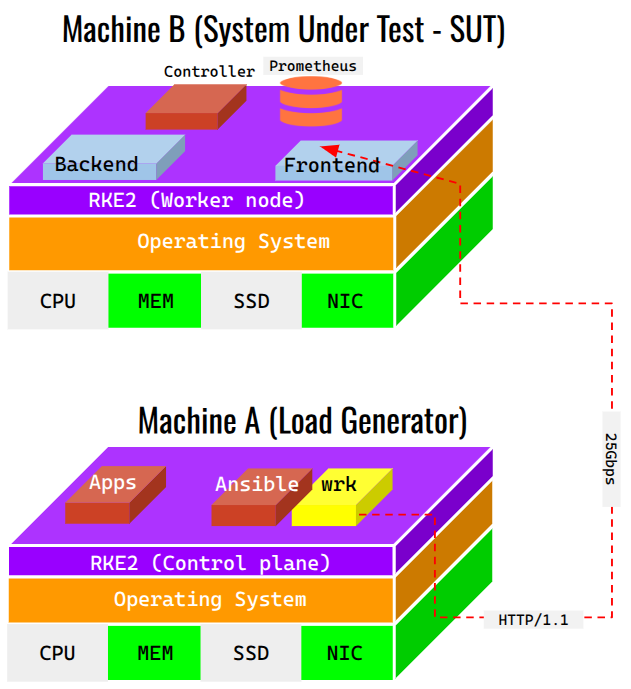
\includegraphics[width=\columnwidth,height=0.3\textheight,keepaspectratio]{fig/topology.png} % or \linewidth
  \caption{Kubernetes cluster environment.}
  \label{fig2}
\end{figure}

\begin{algorithm}
	\caption{Autonomic Controller with Math-based Predictive \& SLA-Aware Dynamic Cutover}
	\label{alg:ctr}
	\begin{algorithmic}[1]
		\STATE \textbf{Inputs:} Poll interval $t_{poll}$, Minimum traffic threshold $\lambda_{min} = 10$, Latency SLA $L_{SLA} = 50$ ms
		\STATE \textbf{Initialize:} $cutover\_triggered \gets \text{False}$
		\WHILE{\textbf{true}}
		\STATE Sleep for $t_{poll}$ seconds
		\IF{$cutover\_triggered = \text{True}$}
		\STATE \textbf{continue} \COMMENT{Idling post-actuation}
		\ENDIF
		\vspace{2mm}
		\STATE \COMMENT{Fetch Real-time Telemetry}
		\STATE $\lambda \gets \text{QueryPrometheus}(\text{Rate of Requests (RPS)})$
		\STATE $S_{cpr} \gets \text{QueryPrometheus}(\text{Average Service Time (s)})$
		\STATE $L_{p95} \gets \text{QueryPrometheus}(\text{App P95 Latency (ms)})$
		\STATE $n_{threads} \gets \text{QueryPrometheus}(\text{Active Threads})$
		
		\IF{$\lambda < \lambda_{min}$ \textbf{or} Telemetry is Null}
		\STATE \textbf{continue} \COMMENT{Wait for stable load}
		\ENDIF
		\vspace{2mm}
		\STATE \COMMENT{Framework Auto-Detection \& Recalibration}
		\IF{$n_{threads} > 50$}
		\STATE $mode \gets \text{SYNC (Flask)}$
		\STATE $c \gets n_{threads}$ \COMMENT{Capacity bounded by OS threads}
		\STATE $\tau_{ratio} $
		\ELSE
		\STATE $mode \gets \text{ASYNC (FastAPI)}$
		\STATE $c \gets n_{async\_event\_loop}$ \COMMENT{Estimated concurrent event loop tasks}
		\STATE $\tau_{ratio} $
		\ENDIF
		\STATE $c \gets 1.0$ \COMMENT{Normalized parallel compute capacity}
		\STATE $\tau_{ratio} \gets 0.80$ \COMMENT{Target utilization threshold}
		\vspace{2mm}
		\STATE \COMMENT{Calculate Queueing Saturation Threshold}
		\STATE $\lambda_{sat} \gets \frac{c}{S_{cpr}}$
		\STATE $\lambda_{trigger} \gets \lambda_{sat} \times \tau_{ratio}$
		\vspace{2mm}
		\STATE \COMMENT{Dual-Condition Evaluation}
		\IF{$\lambda \geq \lambda_{trigger}$ \textbf{and} $L_{p95} \geq L_{SLA}$}
		\STATE $t_{start} \gets \text{CurrentTime}()$
		\STATE $\text{PatchDeployment}(\text{sidecar.istio.io/inject="true"})$
		\STATE $\text{WaitUntilReady}(\text{Deployment Replicas})$
		\STATE $\Delta t_{rollout} \gets \text{CurrentTime}() - t_{start}$
		\STATE $\text{LogActuationMetrics}(\Delta t_{rollout})$
		\STATE $cutover\_triggered \gets \text{True}$
		\ENDIF
		\ENDWHILE
	\end{algorithmic}
\end{algorithm}

%%%%%%%%%%%%%%%%%%%%%%%%%%%%%%%%%%%%%%%%%%%%%%%%%%%%%%%%%%%%%%%%%%%%%%%
\section{Methodology}
\label{sec4}
%%%%%%%%%%%%%%%%%%%%%%%%%%%%%%%%%%%%%%%%%%%%%%%%%%%%%%%%%%%%%%%%%%%%%%%

To validate the proposed mathematical model and pinpoint accurately where latency overhead originates, we conducted controlled experiments in a containerized distributed setting. Our evaluation follows a strict component isolation strategy: we first measure end-to-end performance across the full system and then benchmark the backend service alone in order to distinguish computation time from communication-related delays. This was achieved by deploying a stateless, deterministic backend and enforcing Kubernetes Guaranteed QoS (matching CPU/memory requests to limits) to eliminate resource throttling and "noisy neighbor" interference. 

Our testbed uses a Python WSGI stack (Flask/Gunicorn \cite{gunicorn}) as a standard API gateway. We aim to check how gRPC connection churn impacts performance, not to compare frameworks. Synchronous threads are sensitive to blocking network inputs, highlighting queueing issues.

\begin{figure}
	\centering
	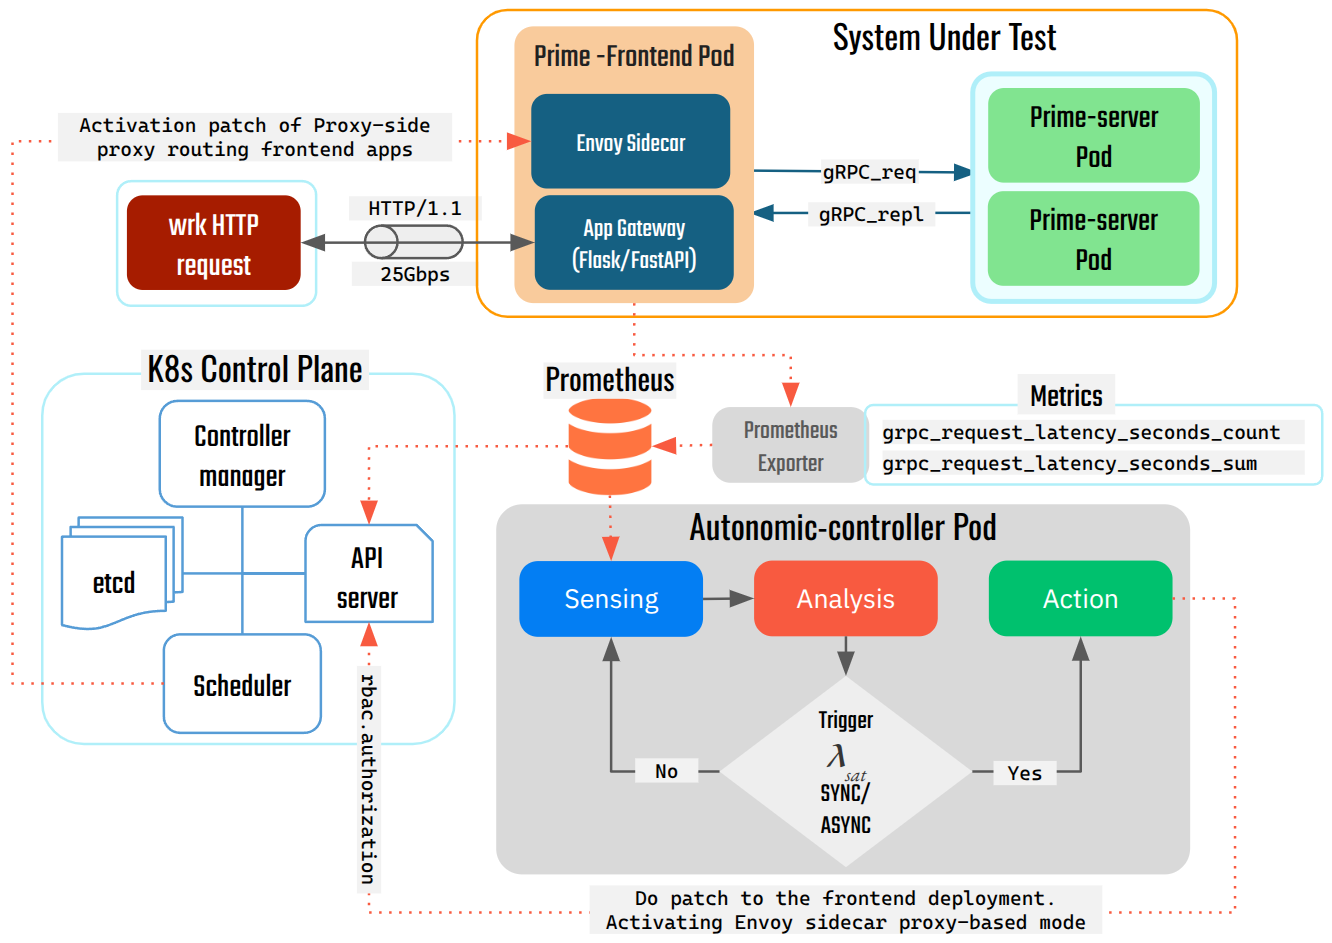
\includegraphics[width=\columnwidth,height=0.25\textheight,keepaspectratio]{fig/ctr-framework.png} % or \linewidth
	\caption{The proactive autonomic controller framework.}
	\label{ctr-frame}
\end{figure}


\subsection{Experimental Environment and Architecture}
\label{sec4.1}

The experiment was conducted on a Kubernetes cluster composed of multiple worker nodes as shown in the Fig. \ref{fig2}. The system under test (SUT) consists of two main microservice components:

\begin{itemize}
    \item \textbf{gRPC Backend Service (prime-server)}: A high-performance Python application responsible for CPU-intensive prime number verification. To eliminate backend capacity as a confounding variable, this component was over-provisioned with 10 identical replica pods, deployed behind a Kubernetes NodePort Service.

    \item \textbf{API Gateway (prime-frontend)}: A Python Flask application running within Gunicorn workers. This component acts as an HTTP/REST to gRPC proxy. It was strictly limited to 2 replica pods to intentionally force saturation and observe gateway-tier queuing dynamics under heavy load. 
\end{itemize}

\subsection{Workload Generation and Component Isolation}
\label{4.2}


To precisely calculate the application-layer gateway overhead, we utilized two specialized, open-source load-testing tools (\textit{wrk2} \cite{wrk2} and \textit{ghz} \cite{ghz}), as shown in the Fig. \ref{fig3}:

\begin{itemize}
    \item \textbf{Unoptimized Gateway (CPR):} Simulates Algorithm~\ref{alg1} ($mode = \text{CPR}$), forcing TCP/HTTP2 renegotiation for every incoming request.
    \item \textbf{Optimized Gateway (PCR):} Simulates Algorithm~\ref{alg1} ($mode = \text{PCR}$), routing concurrent accesses through a single, globally initialized gRPC channel.
\end{itemize}


Both tools executed 30 iterations for each target throughput level (ranging from 100 to 1000 Requests Per Second, or RPS), sustaining the load for 60 seconds per iteration to allow queueing buffers to stabilize.

%%%%%%%%%%%%%%%%%%%%%%%%%%%%%%%%%%%%%%%%%%%%%%%%%%%%%%%%%%%%%%%%%%%%%%%
\section{Results and Discussion}
\label{sec5}
%%%%%%%%%%%%%%%%%%%%%%%%%%%%%%%%%%%%%%%%%%%%%%%%%%%%%%%%%%%%%%%%%%%%%%%

The empirical results have successfully proven that the predicted Asymptotic latency degradation is caused by the $M/M/c$ queuing model in the Connection-Per-Request (CPR) paradigm and have clearly demonstrated the transformational impact of Persistent Channel Reuse (PCR). 

\subsection{Baseline: Backend gRPC Performance}
\label{sec5.1}

%\begin{figure}
%  \centering
%  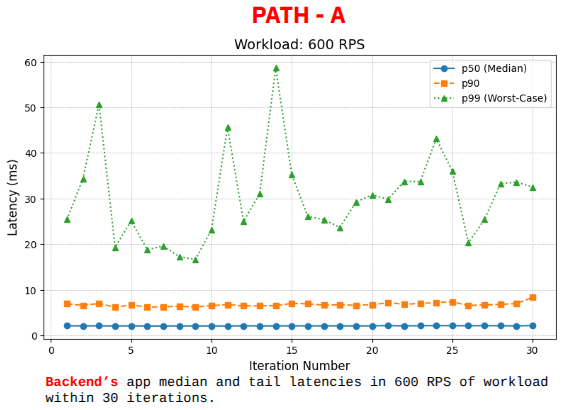
\includegraphics[width=\columnwidth,height=0.23\textheight,keepaspectratio]{fig/result2.png} % or \linewidth
%  \caption{gRPC backend latency evaluation using ghz benchmark tool.}
%  \label{fig4}
%\end{figure}

%\begin{figure}
%  \centering
%  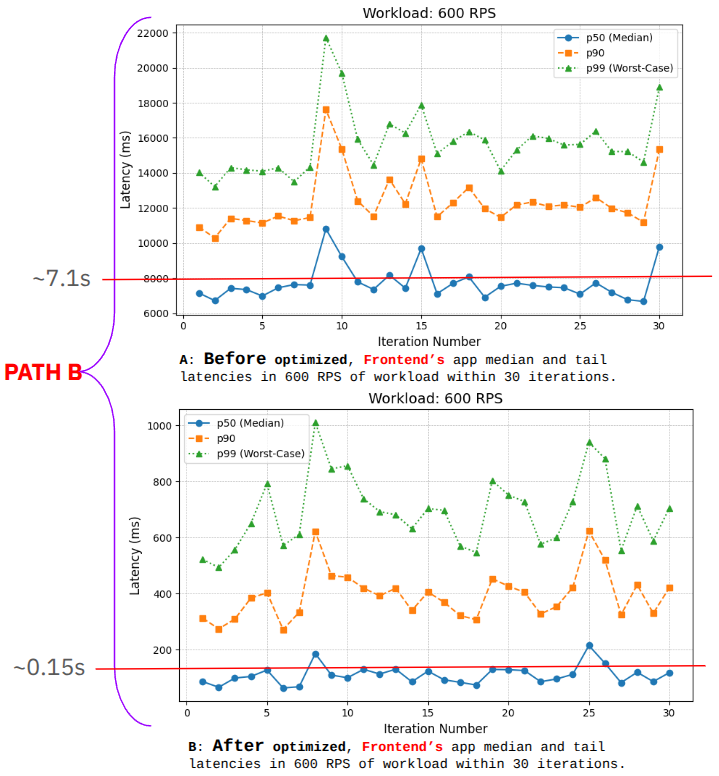
\includegraphics[width=\columnwidth,height=0.35\textheight,keepaspectratio]{fig/result1.png} % or \linewidth
%  \caption{End-to-end frontend latency evaluation using wrk2 as workload generator. (A) Connection-Per-Request paradigm - \textbf{Before} optimized, (B) Persistent Channel Reuse paradigm - \textbf{After} optimized}
%  \label{fig5}
%\end{figure}

The ghz test results established an exceptional and highly stable baseline. Across the entire load spectrum (100 to 1000 RPS), the 10 prime-server backend pods consistently delivered a median (p50) latency of $\sim 2.5 \text{ ms} \text{ to } 3.6 \text{ ms}$, with p90 latencies remaining firmly under 10 ms. 

This flat latency curve definitively proved that the backend architecture was not the system bottleneck, as shown in the Fig. \ref{fig4}. By having 10 backend pods, we mathematically guaranteed that the backend possessed vastly more computational capacity than the frontend could ever saturate. The computational capacity of the prime number verification logic was highly resilient, isolating the source of any overarching performance degradation to the gateway tier.

\textbf{Concurrency Configuration and Multiplexing:}
During empirical testing, both \textit{ghz} and \textit{wrk2} were configured to simulate high concurrency using a fixed pool of 50 simultaneous client connections across all target throughput levels ($\lambda$). It is critical to note how these concurrent accesses are handled internally by the optimized gateway. Under the PCR paradigm, the concurrent requests arriving at the gateway are not queued sequentially over the network; instead, the underlying gRPC framework maps these concurrent application-level accesses into discrete, parallel HTTP/2 streams over a \textit{single} shared TCP connection. This mechanism prevents connection exhaustion and directly validates our mathematical assumption that $S_{pcr}$ approaches pure RPC execution time without queuing at the network socket layer.

\subsection{Unoptimized System: The CPR Bottleneck}
\label{sec5.2}

Testing the end-to-end system utilizing the CPR paradigm revealed a catastrophic bottleneck, as shown in the Fig. \ref{fig5}-A (upper side). At a moderate load of 400 RPS, the system maintained a median latency of $\sim 400 \text{ ms}$. However, as throughput increased to 600 RPS, the system hit the critical utilization threshold ($\rho \to 1$).

Median latency exploded to $> 7,100 \text{ ms}$, and p99 latency spiked past $14,000 \text{ ms}$. This exponential degradation perfectly aligns with the queueing theory model where service time ($S_{cpr}$) is artificially inflated by excessive TCP/HTTP2 handshake overheads for every transaction. The gateway workers were entirely occupied managing network state rather than processing business logic.

\subsection{Optimized System: PCR Implementation}
\label{sec5.3}

By deploying the algorithmic optimization detailed in Section \ref{sec3} (establishing a persistent, multiplexed gRPC channel at application startup - Algorithm \ref{alg1}), the performance profile of the system was qualitatively transformed.

At 600 RPS, the optimized system recorded a median latency of $\sim 150 \text{ ms}$, as shown in the Fig. \ref{fig5}-B (lower side). This represents a $\sim 97.9\%$ reduction in end-to-end latency compared to the CPR paradigm. Furthermore, the system successfully sustained loads up to 800 RPS before demonstrating signs of stress, effectively doubling the system's maximum throughput capacity without provisioning any additional infrastructure resources.

\subsection{Quantifying the Inherent Proxy Latency Gap}
\label{sec5.4}

By subtracting the baseline backend network latency ($T_{network}$) established via \textit{ghz} from the full end-to-end system latency ($T_{total}$) measured via \textit{wrk2}, we can isolate the underlying application-layer tax. We define this remaining overhead as the Inherent Proxy Latency Gap---the baseline latency strictly attributable to the framework's internal request handling, independent of network state management.

%\begin{table}[htbp]
%   \centering
%    \caption{\textbf{Comparative Latency Overhead at Optimal Saturation Point (400 RPS)}}
%   \label{table1}
%   \resizebox{\columnwidth}{!}{% <--- This scales the table to the column width
%    \begin{tabular}{lcc}
%    \toprule
%    \textbf{Component Level} & \textbf{Median Latency (p50)} & \textbf{Percentage of Total Latency} \\ \midrule
%    Backend Only (\textit{ghz}) & $\sim 2.8$ ms & 2.5\% \\
%    Full System (CPR, Before) & $\sim 400$ ms & 100\% \\
%    Full System (PCR, After) & \textbf{$\sim 110$ ms} & \textbf{100\%} \\ \midrule
%    \textbf{Gateway Overhead (PCR)} & \textbf{$\sim 107.2$ ms} & \textbf{97.5\%} \\ \bottomrule
%    \end{tabular}%
%    }
%\end{table}

\begin{table}[htbp]
\centering
\caption{\textbf{Comparative Latency Overhead at Optimal Saturation Point (400 RPS)}}
\label{table1}
\setlength{\tabcolsep}{3pt}
%\resizebox{\columnwidth}{!}{
%\begin{tabular}{|p{110pt}|p{75pt}|p{100pt}|}
\begin{tabular}{lcc}
\hline
\textbf{Component level}& \textbf{Median latency (p50)}& \textbf{Percentage of total latency}\\
\hline
Backend Only (\textit{ghz}) & $\sim 2.8$ ms & 2.5\% \\
Full System (CPR, Before) & $\sim 400$ ms & 100\% \\
Full System (PCR, After) & $\sim 110$ ms & 100\% \\
\hline
\textbf{Gateway Overhead (PCR)} & $\sim 107.2$ ms & 97.5\% \\ 
\hline
%}
\end{tabular}
\end{table}
    
As illustrated in Table~\ref{table1}, the results reveal a compelling paradox in the optimized PCR paradigm. Although the persistent channel implementation successfully averted queue saturation and achieved a 97\% reduction in total latency compared to the CPR baseline, a compositional analysis shows that the gateway tier still accounts for 97.5\% of the remaining end-to-end response time. 

This empirical gap directly connects our theoretical approach to the user experience. In our PCR model, the actual backend computational execution ($T_{network}$) requires only $\sim 2.8$ ms ($2.5\%$ of total time), while the remaining $107.2$ ms is consumed by the gateway. Critically, this gap encompasses not only the Python WSGI \cite{wsgi-pep} stack execution but also the protocol transcoding overhead—the computational cost of parsing incoming HTTP/1.1 JSON requests from \textit{wrk2} and serializing them into HTTP/2 Protobuf messages for the gRPC backend. 

This reveals a fundamental "Performance-Abstraction Paradox." While developers utilize API gateways to seamlessly bridge RESTful clients (HTTP/1.1) with high-performance microservices (gRPC), this protocol translation introduces a structural latency tax that dwarfs the business logic itself. Consequently, while our PCR optimization resolves protocol-level queue saturation, the absolute lower bound of system latency remains strictly dictated by the gateway's HTTP-to-gRPC transcoding efficiency.

\subsection{Empirical Validation of the Queueing Model}

To rigorously evaluate the mathematical framework proposed in Section \ref{sec2}, we mapped our empirical throughput and latency data to the $M/M/c$ queueing model. Our objective was to prove that the catastrophic latency spikes observed were not random system failures, but rather predictable queuing saturation events driven by connection churn.

In our system architecture, the gateway tier acts as the server pool ($c$ workers). The arrival rate of incoming requests is defined as $\lambda$ (varying from 100 to 1000 RPS). The service rate of the gateway, $\mu$, is inversely proportional to the service time ($S_{gateway}$). 

Under the Connection-Per-Request (CPR) paradigm, the service time ($S_{cpr}$) includes the mandatory TCP and HTTP/2 handshakes ($t_{tcp} + t_{http2}$). Because these network operations block gateway worker threads, $\mu_{cpr}$ is severely restricted. 

Our empirical data aligns perfectly with the theoretical utilization formula: 
$$
\rho = \frac{\lambda}{c \cdot \mu}
$$

According to Little's Law \cite{little2011or}, queueing delay $W_{queue}$ grows asymptotically as system utilization $\rho \to 1$:
$$
W_{queue} \propto \frac{\rho}{1 - \rho}
$$

\textbf{Evaluating the CPR Saturation Point:}
During our baseline CPR testing, the system maintained a median latency of $\sim 400 \text{ ms}$ at $\lambda = 400 \text{ RPS}$, indicating high but stable utilization ($\rho < 1$). However, when the arrival rate increased to $\lambda = 600 \text{ RPS}$, the median latency violently spiked to $> 7,100 \text{ ms}$. This exponential degradation confirms that the low service rate ($\mu_{cpr}$) caused the gateway to cross the critical threshold of $\rho = 1$ at a mere 600 RPS. At this point, requests were arriving faster than connections could be negotiated, causing $W_{queue}$ to theoretically approach infinity, which manifested empirically as 7-second tail latencies and connection timeouts.

\textbf{Evaluating the PCR Optimization:}
By transitioning to the Persistent Channel Reuse (PCR) paradigm, we eliminated the handshake overhead, drastically reducing the service time to $S_{pcr}$ and thereby significantly increasing the service rate ($\mu_{pcr}$). Because $\mu_{pcr} \gg \mu_{cpr}$, the utilization $\rho$ at the same arrival rate ($\lambda = 600 \text{ RPS}$) remained well below 1. 

To clarify the protocol dynamics, the Persistent Channel Reuse (PCR) approach does not reimplement HTTP/2 features; rather, it maintains a single global TCP session to allow native HTTP/2 stream multiplexing to function as intended. Conversely, the CPR anti-pattern actively sabotages this multiplexing capability by forcing the underlying library to establish and destroy a unique TCP session for every individual request.

Consequently, the queueing delay $W_{queue}$ collapsed. The empirical result—a drop in latency from $> 7,100 \text{ ms}$ to exactly $150 \text{ ms}$ at 600 RPS—serves as a direct physical validation of the $M/M/c$ model. It proves that correcting the $O(N)$ connection anti-pattern artificially scales the service rate $\mu$, averting queue saturation without provisioning any additional hardware capacity ($c$).

%%%%%%%%%%%%%%%%%%%%%%%%%%%%%%%%%%%%%%%%%%%%%%%%%%%%%%%%%%%%%%%%%%%%%%%
\section{Conclusion and Future Work}
\label{sec6}
%%%%%%%%%%%%%%%%%%%%%%%%%%%%%%%%%%%%%%%%%%%%%%%%%%%%%%%%%%%%%%%%%%%%%%%

In this paper, we investigated the hidden performance costs of application-layer communication bottlenecks in microservice architectures, focusing on the gRPC connection churn flaw within API gateways. We modeled the request patterns of the "connection-per-request" (CPR) anti-pattern and contrasted it with a refactored Persistent Channel Reuse (PCR) approach. The observation of actual runs demonstrated that refactoring the gateway implementation to the PCR approach yielded a 97\% reduction in median system latency—dropping from over 7,100 ms to 150 ms under a peak load of 600 RPS. This study proves that correcting application-layer protocol mismanagement successfully moves the performance bottleneck away from the infrastructure gateway and to the compute backend, highlighting that refactoring the gateway code is a critical aspect to scalability as the underlying architectural design.

Future work will expand this steady-state benchmarking methodology into the domain of Chaos Engineering. By introducing controlled faults (e.g., node resource starvation, sudden pod termination) under a persistent load. 

\section{\break Submitting Your Paper for Review}

\subsection{Final Stage}
When your article is accepted, you can submit the final files, including figures, tables, and photos, per the journal's guidelines through the submission system used to submit the articlle.
 You may use \emph{Zip} for large files, or compress files using \emph{Compress, Pkzip, Stuffit,} or \emph{Gzip.}

In addition, designate one author as the ``corresponding author.'' This is the author to
whom proofs of the paper will be sent. Proofs are sent to the corresponding
author only.

\subsection{Review Stage Using IEEE Author Portal}
Article contributions to IEEE Access should be submitted electronically on the IEEE Author Portal. For more information, please visit
\underline{https://ieeeaccess.ieee.org/}.

Along with other information, you will be asked to select the subject from a
pull-down list. There are various steps to the
submission process; you must complete all steps for a complete submission.
At the end of each step you must click ``Save and Continue''; just uploading
the paper is not sufficient. After the last step, you should see a
confirmation that the submission is complete. You should also receive an
e-mail confirmation. For inquiries regarding the submission of your article, please contact ieeeaccess@ieee.org.

The manuscript should be prepared in a double column, single-spaced format using a required IEEE Access template.
A Word or LaTeX file and a PDF file are both required upon submission in the IEEE Author Portal.

\subsection{Final Stage Using IEEE Author Portal}
Upon acceptance, you will receive an email with specific instructions

Designate the author who submitted the manuscript on
IEEE Author Portal as the ``corresponding author.'' This is the only
author to whom proofs of the paper will be sent.

\subsection{Copyright Form}
Authors must submit an electronic IEEE Copyright Form (eCF) upon submitting
their final manuscript files. You can access the eCF system through your
manuscript submission system or through the Author Gateway. You are
responsible for obtaining any necessary approvals and/or security
clearances. For additional information on intellectual property rights,
visit the IEEE Intellectual Property Rights department web page at
\underline{http://www.ieee.org/publications\_standards/publications/}\break\underline{rights/index.html}.

\section{\break IEEE Publishing Policy}
The general IEEE policy requires that authors should only submit original
work that has neither appeared elsewhere for publication, nor is under
review for another refereed publication. The submitting author must disclose
all prior publication(s) and current submissions when submitting a
manuscript. Do not publish ``preliminary'' data or results. To avoid any delays in
publication, please be sure to follow these instructions.  Final
submissions should include source files of your accepted manuscript, high
quality graphic files, and a formatted pdf file. If you have any questions
regarding the final submission process, please contact the administrative
contact for the journal.
author is responsible for obtaining agreement of all coauthors and any
consent required from employers or sponsors before submitting an article.

The IEEE Access Editorial Office does not publish conference
records or proceedings, but can publish articles related to conferences that
have undergone rigorous peer review. Minimally, two reviews are required for
every article submitted for peer review.

\section{\break Publication Principles}
Authors should consider the following points:

\begin{enumerate}
\item Technical papers submitted for publication must advance the state of knowledge and must cite relevant prior work.
\item The length of a submitted paper should be commensurate with the importance, or appropriate to the complexity, of the work. For example, an obvious extension of previously published work might not be appropriate for publication or might be adequately treated in just a few pages.
\item Authors must convince both peer reviewers and the editors of the scientific and technical merit of a paper; the standards of proof are higher when extraordinary or unexpected results are reported.
\item Because replication is required for scientific progress, papers submitted for publication must provide sufficient information to allow readers to perform similar experiments or calculations and
use the reported results. Although not everything need be disclosed, a paper
must contain new, useable, and fully described information. For example, a
specimen's chemical composition need not be reported if the main purpose of
a paper is to introduce a new measurement technique. Authors should expect
to be challenged by reviewers if the results are not supported by adequate
data and critical details.
\item Papers that describe ongoing work or announce the latest technical achievement, which are suitable for presentation at a professional conference, may not be appropriate for publication.
\end{enumerate}



\section{\break Reference Examples}

\begin{itemize}

\item \emph{Basic format for books:}\\
J. K. Author, ``Title of chapter in the book,'' in \emph{Title of His Published Book, x}th ed. City of Publisher, (only U.S. State), Country: Abbrev. of Publisher, year, ch. $x$, sec. $x$, pp. \emph{xxx--xxx.}\\
See \cite{b1,b2}.

\item \emph{Basic format for periodicals:}\\
J. K. Author, ``Name of paper,'' \emph{Abbrev. Title of Periodical}, vol. \emph{x, no}. $x, $pp\emph{. xxx--xxx, }Abbrev. Month, year, DOI. 10.1109.\emph{XXX}.123456.\\
See \cite{b3}--\cite{b5}.

\item \emph{Basic format for reports:}\\
J. K. Author, ``Title of report,'' Abbrev. Name of Co., City of Co., Abbrev. State, Country, Rep. \emph{xxx}, year.\\
See \cite{b6,b7}.

\item \emph{Basic format for handbooks:}\\
\emph{Name of Manual/Handbook, x} ed., Abbrev. Name of Co., City of Co., Abbrev. State, Country, year, pp. \emph{xxx--xxx.}\\
See \cite{b8,b9}.

\item \emph{Basic format for books (when available online):}\\
J. K. Author, ``Title of chapter in the book,'' in \emph{Title of
Published Book}, $x$th ed. City of Publisher, State, Country: Abbrev.
of Publisher, year, ch. $x$, sec. $x$, pp. \emph{xxx--xxx}. [Online].
Available: \underline{http://www.web.com}\\
See \cite{b10}--\cite{b13}.

\item \emph{Basic format for journals (when available online):}\\
J. K. Author, ``Name of paper,'' \emph{Abbrev. Title of Periodical}, vol. $x$, no. $x$, pp. \emph{xxx--xxx}, Abbrev. Month, year. Accessed on: Month, Day, year, DOI: 10.1109.\emph{XXX}.123456, [Online].\\
See \cite{b14}--\cite{b16}.

\item \emph{Basic format for papers presented at conferences (when available online): }\\
J.K. Author. (year, month). Title. presented at abbrev. conference title. [Type of Medium]. Available: site/path/file\\
See \cite{b17}.

\item \emph{Basic format for reports and handbooks (when available online):}\\
J. K. Author. ``Title of report,'' Company. City, State, Country. Rep. no., (optional: vol./issue), Date. [Online] Available: site/path/file\\
See \cite{b18,b19}.

\item \emph{Basic format for computer programs and electronic documents (when available online): }\\
Legislative body. Number of Congress, Session. (year, month day). \emph{Number of bill or resolution}, \emph{Title}. [Type of medium]. Available: site/path/file\\
See \cite{b20}.

\item \emph{Basic format for patents (when available online):}\\
Name of the invention, by inventor's name. (year, month day). Patent Number [Type of medium]. Available: site/path/file\\
See \cite{b21}.

\item \emph{Basic format}\emph{for conference proceedings (published):}\\
J. K. Author, ``Title of paper,'' in \emph{Abbreviated Name of Conf.}, City of Conf., Abbrev. State (if given), Country, year, pp. \emph{xxxxxx.}\\
See \cite{b22}.

\item \emph{Example for papers presented at conferences (unpublished):}\\
See \cite{b23}.

\item \emph{Basic format for patents}$:$\\
J. K. Author, ``Title of patent,'' U.S. Patent \emph{x xxx xxx}, Abbrev. Month, day, year.\\
See \cite{b24}.

\item \emph{Basic format for theses (M.S.) and dissertations (Ph.D.):}
\begin{enumerate}
\item J. K. Author, ``Title of thesis,'' M.S. thesis, Abbrev. Dept., Abbrev. Univ., City of Univ., Abbrev. State, year.
\item J. K. Author, ``Title of dissertation,'' Ph.D. dissertation, Abbrev. Dept., Abbrev. Univ., City of Univ., Abbrev. State, year.
\end{enumerate}
See \cite{b25,b26}.

\item \emph{Basic format for the most common types of unpublished references:}
\begin{enumerate}
\item J. K. Author, private communication, Abbrev. Month, year.
\item J. K. Author, ``Title of paper,'' unpublished.
\item J. K. Author, ``Title of paper,'' to be published.
\end{enumerate}
See \cite{b27}--\cite{b29}.

\item \emph{Basic formats for standards:}
\begin{enumerate}
\item \emph{Title of Standard}, Standard number, date.
\item \emph{Title of Standard}, Standard number, Corporate author, location, date.
\end{enumerate}
See \cite{b30,b31}.

\item \emph{Article number in~reference examples:}\\
See \cite{b32,b33}.

\item \emph{Example when using et al.:}\\
See \cite{b34}.

\end{itemize}


\section*{Acknowledgment}
The preferred spelling of the word ``acknowledgment'' in American English is
without an ``e'' after the ``g.'' Use the singular heading even if you have
many acknowledgments. Avoid expressions such as ``One of us (S.B.A.) would
like to thank $\ldots$ .'' Instead, write ``F. A. Author thanks $\ldots$ .'' In most
cases, sponsor and financial support acknowledgments are placed in the
unnumbered footnote on the first page, not here.


\begin{thebibliography}{00}

\bibitem{martin2022online} A. Martin-Lopez, S. Segura, and A. Ruiz-Cortés, ``Online testing of RESTful APIs: Promises and challenges,'' in Proc. 30th ACM Joint Eur. Softw. Eng. Conf. Symp. Found. Softw. Eng., 2022, pp. 408--420.

\bibitem{Ventre2018SDNAAA} P. L. Ventre, M. M. Tajiki, S. Salsano, and C. Filsfils, ``SDN architecture and southbound APIs for IPv6 segment routing enabled wide area networks,'' IEEE Trans. Netw. Service Manag., vol. 15, pp. 1378--1392, 2018.

\bibitem{zhu2023dissecting} X. Zhu, G. She, B. Xue, Y. Zhang, Y. Zhang, X. K. Zou, X. Duan, P. He, A. Krishnamurthy, and M. Lentz, ``Dissecting overheads of service mesh sidecars,'' in Proc. 2023 ACM Symp. Cloud Comput., 2023, pp. 142--157.

\bibitem{Guo2020StatefulTCPANAA} L. Guo and J. Y. B. Lee, ``Stateful-TCP—a new approach to accelerate TCP slow-start,'' IEEE Access, vol. 8, pp. 195955--195970, 2020.

\bibitem{pinheiro2024performance} T. Pinheiro, M. Mialaret, P. Pereira, L. Lins, D. Silva, J. Dantas, and P. Maciel, ``Performance modeling of microservices with circuit breakers using stochastic Petri nets,'' in Proc. 2024 IEEE Int. Syst. Conf. (SysCon), 2024, pp. 1--8.

\bibitem{DAuria2021AnMQA} B. D'Auria, I. Adan, R. Bekker, and V. Kulkarni, ``An M/M/c queue with queueing-time dependent service rates,'' Eur. J. Oper. Res., vol. 299, pp. 566--579, 2021.

\bibitem{little2011or} J. D. C. Little, ``OR forum—Little's law as viewed on its 50th anniversary,'' Oper. Res., vol. 59, no. 3, pp. 536--549, 2011.

\bibitem{gunicorn} Gunicorn, ``Gunicorn: Serve Python on the Web.'' [Online]. Available: https://gunicorn.org/. [Accessed: May 14, 2026].

\bibitem{wsgi-pep} P. J. Eby, ``PEP 333 – Python Web Server Gateway Interface v1.0,'' Sep. 27, 2010. [Online]. Available: https://peps.python.org/pep-0333/. [Accessed: Apr. 23, 2026].

\bibitem{wrk2} G. Tene, ``A HTTP benchmarking tool based mostly on wrk,'' Jun. 28, 2016. [Online]. Available: https://github.com/giltene/wrk2. [Accessed: May 14, 2026].

\bibitem{ghz} B. Djurkovic, ``gRPC benchmarking and load testing tool,'' Dec. 7, 2025. [Online]. Available: https://github.com/bojand/ghz. [Accessed: May 14, 2026].

\bibitem{tijms2003first} H. C. Tijms, \textit{A first course in stochastic models}, vol. 2, Wiley New York, 2003.

\bibitem{Banerjee2023MTDDHJSMTA} P. Banerjee, S. Roy, A. Sinha, M. Hassan, S. Burje, A. Agrawal, A. K. Bairagi, S. Alshathri, and W. El-shafai, "MTD-DHJS: Makespan-Optimized Task Scheduling Algorithm for Cloud Computing With Dynamic Computational Time Prediction," \textit{IEEE Access}, vol. 11, pp. 105578--105618, 2023.




\bibitem{b1} G. O. Young, ``Synthetic structure of industrial plastics,'' in \emph{Plastics,} 2\textsuperscript{nd} ed., vol. 3, J. Peters, Ed. New York, NY, USA: McGraw-Hill, 1964, pp. 15--64.

\bibitem{b2} W.-K. Chen, \emph{Linear Networks and Systems.} Belmont, CA, USA: Wadsworth, 1993, pp. 123--135.

\bibitem{b3} J. U. Duncombe, ``Infrared navigation---Part I: An assessment of feasibility,'' \emph{IEEE Trans. Electron Devices}, vol. ED-11, no. 1, pp. 34--39, Jan. 1959, 10.1109/TED.2016.2628402.

\bibitem{b4} E. P. Wigner, ``Theory of traveling-wave optical laser,'' \emph{Phys. Rev}., vol. 134, pp. A635--A646, Dec. 1965.

\bibitem{b5} E. H. Miller, ``A note on reflector arrays,'' \emph{IEEE Trans. Antennas Propagat}., to be published.

\bibitem{b6} E. E. Reber, R. L. Michell, and C. J. Carter, ``Oxygen absorption in the earth's atmosphere,'' Aerospace Corp., Los Angeles, CA, USA, Tech. Rep. TR-0200 (4230-46)-3, Nov. 1988.

\bibitem{b7} J. H. Davis and J. R. Cogdell, ``Calibration program for the 16-foot antenna,'' Elect. Eng. Res. Lab., Univ. Texas, Austin, TX, USA, Tech. Memo. NGL-006-69-3, Nov. 15, 1987.

\bibitem{b8} \emph{Transmission Systems for Communications}, 3\textsuperscript{rd} ed., Western Electric Co., Winston-Salem, NC, USA, 1985, pp. 44--60.

\bibitem{b9} \emph{Motorola Semiconductor Data Manual}, Motorola Semiconductor Products Inc., Phoenix, AZ, USA, 1989.

\bibitem{b10} G. O. Young, ``Synthetic structure of industrial
plastics,'' in Plastics, vol. 3, Polymers of Hexadromicon, J. Peters,
Ed., 2\textsuperscript{nd} ed. New York, NY, USA: McGraw-Hill, 1964, pp. 15-64.
[Online]. Available:
\underline{http://www.bookref.com}.

\bibitem{b11} \emph{The Founders' Constitution}, Philip B. Kurland
and Ralph Lerner, eds., Chicago, IL, USA: Univ. Chicago Press, 1987.
[Online]. Available: \underline{http://press-pubs.uchicago.edu/founders/}

\bibitem{b12} The Terahertz Wave eBook. ZOmega Terahertz Corp., 2014.
[Online]. Available:
\underline{http://dl.z-thz.com/eBook/zomegaebookpdf\_1206\_sr.pdf}. Accessed on: May 19, 2014.

\bibitem{b13} Philip B. Kurland and Ralph Lerner, eds., \emph{The
Founders' Constitution.} Chicago, IL, USA: Univ. of Chicago Press,
1987, Accessed on: Feb. 28, 2010, [Online] Available:
\underline{http://press-pubs.uchicago.edu/founders/}

\bibitem{b14} J. S. Turner, ``New directions in communications,'' \emph{IEEE J. Sel. Areas Commun}., vol. 13, no. 1, pp. 11-23, Jan. 1995.

\bibitem{b15} W. P. Risk, G. S. Kino, and H. J. Shaw, ``Fiber-optic frequency shifter using a surface acoustic wave incident at an oblique angle,'' \emph{Opt. Lett.}, vol. 11, no. 2, pp. 115--117, Feb. 1986.

\bibitem{b16} P. Kopyt \emph{et al., ``}Electric properties of graphene-based conductive layers from DC up to terahertz range,'' \emph{IEEE THz Sci. Technol.,} to be published. DOI: 10.1109/TTHZ.2016.2544142.

\bibitem{b17} PROCESS Corporation, Boston, MA, USA. Intranets:
Internet technologies deployed behind the firewall for corporate
productivity. Presented at INET96 Annual Meeting. [Online].
Available: \underline{http://home.process.com/Intranets/wp2.htp}

\bibitem{b18} R. J. Hijmans and J. van Etten, ``Raster: Geographic analysis and modeling with raster data,'' R Package Version 2.0-12, Jan. 12, 2012. [Online]. Available: \underline {http://CRAN.R-project.org/package=raster}

\bibitem{b19} Teralyzer. Lytera UG, Kirchhain, Germany [Online].
Available:
\underline{http://www.lytera.de/Terahertz\_THz\_Spectroscopy.php?id=home}, Accessed on: Jun. 5, 2014.

\bibitem{b20} U.S. House. 102\textsuperscript{nd} Congress, 1\textsuperscript{st} Session. (1991, Jan. 11). \emph{H. Con. Res. 1, Sense of the Congress on Approval of}  \emph{Military Action}. [Online]. Available: LEXIS Library: GENFED File: BILLS

\bibitem{b21} Musical toothbrush with mirror, by L.M.R. Brooks. (1992, May 19). Patent D 326 189 [Online]. Available: NEXIS Library: LEXPAT File: DES

\bibitem{b22} D. B. Payne and J. R. Stern, ``Wavelength-switched pas- sively coupled single-mode optical network,'' in \emph{Proc. IOOC-ECOC,} Boston, MA, USA, 1985, pp. 585--590.

\bibitem{b23} D. Ebehard and E. Voges, ``Digital single sideband detection for interferometric sensors,'' presented at the \emph{2\textsuperscript{nd} Int. Conf. Optical Fiber Sensors,} Stuttgart, Germany, Jan. 2-5, 1984.

\bibitem{b24} G. Brandli and M. Dick, ``Alternating current fed power supply,'' U.S. Patent 4 084 217, Nov. 4, 1978.

\bibitem{b25} J. O. Williams, ``Narrow-band analyzer,'' Ph.D. dissertation, Dept. Elect. Eng., Harvard Univ., Cambridge, MA, USA, 1993.

\bibitem{b26} N. Kawasaki, ``Parametric study of thermal and chemical nonequilibrium nozzle flow,'' M.S. thesis, Dept. Electron. Eng., Osaka Univ., Osaka, Japan, 1993.

\bibitem{b27} A. Harrison, private communication, May 1995.

\bibitem{b28} B. Smith, ``An approach to graphs of linear forms,'' unpublished.

\bibitem{b29} A. Brahms, ``Representation error for real numbers in binary computer arithmetic,'' IEEE Computer Group Repository, Paper R-67-85.

\bibitem{b30} IEEE Criteria for Class IE Electric Systems, IEEE Standard 308, 1969.

\bibitem{b31} Letter Symbols for Quantities, ANSI Standard Y10.5-1968.

\bibitem{b32} R. Fardel, M. Nagel, F. Nuesch, T. Lippert, and A. Wokaun, ``Fabrication of organic light emitting diode pixels by laser-assisted forward transfer,'' \emph{Appl. Phys. Lett.}, vol. 91, no. 6, Aug. 2007, Art. no. 061103.~

\bibitem{b33} J. Zhang and N. Tansu, ``Optical gain and laser characteristics of InGaN quantum wells on ternary InGaN substrates,'' \emph{IEEE Photon. J.}, vol. 5, no. 2, Apr. 2013, Art. no. 2600111

\bibitem{b34} S. Azodolmolky~\emph{et al.}, Experimental demonstration of an impairment aware network planning and operation tool for transparent/translucent optical networks,''~\emph{J. Lightw. Technol.}, vol. 29, no. 4, pp. 439--448, Sep. 2011.

\end{thebibliography}

\begin{IEEEbiography}[{
\includegraphics[width=1in,height=1.25in,clip,keepaspectratio]{author1.png}}]{First A. Author} received the B.S. and M.S. degrees in aerospace engineering from
the University of Virginia, Charlottesville, in 2001 and the Ph.D. degree in
mechanical engineering from Drexel University, Philadelphia, PA, in 2008.

From 2001 to 2004, he was a Research Assistant with the Princeton Plasma
Physics Laboratory. Since 2009, he has been an Assistant Professor with the
Mechanical Engineering Department, Texas A{\&}M University, College Station.
He is the author of three books, more than 150 articles, and more than 70
inventions. His research interests include high-pressure and high-density
nonthermal plasma discharge processes and applications, microscale plasma
discharges, discharges in liquids, spectroscopic diagnostics, plasma
propulsion, and innovation plasma applications. He is an Associate Editor of
the journal \emph{Earth, Moon, Planets}, and holds two patents.

Dr. Author was a recipient of the International Association of Geomagnetism
and Aeronomy Young Scientist Award for Excellence in 2008, and the IEEE
Electromagnetic Compatibility Society Best Symposium Paper Award in 2011.
\end{IEEEbiography}


\begin{IEEEbiography}[{
\includegraphics[width=1in,height=1.25in,clip,keepaspectratio]{author2.png}}]{Second B. Author} (M'76--SM'81--F'87) and all authors may include
biographies. Biographies are often not included in conference-related
papers. This author became a Member (M) of IEEE in 1976, a Senior
Member (SM) in 1981, and a Fellow (F) in 1987. The first paragraph may
contain a place and/or date of birth (list place, then date). Next,
the author's educational background is listed. The degrees should be
listed with type of degree in what field, which institution, city,
state, and country, and year the degree was earned. The author's major
field of study should be lower-cased.

The second paragraph uses the pronoun of the person (he or she) and not the
author's last name. It lists military and work experience, including summer
and fellowship jobs. Job titles are capitalized. The current job must have a
location; previous positions may be listed
without one. Information concerning previous publications may be included.
Try not to list more than three books or published articles. The format for
listing publishers of a book within the biography is: title of book
(publisher name, year) similar to a reference. Current and previous research
interests end the paragraph.

The third paragraph begins with the author's
title and last name (e.g., Dr.\ Smith, Prof.\ Jones, Mr.\ Kajor, Ms.\ Hunter).
List any memberships in professional societies other than the IEEE. Finally,
list any awards and work for IEEE committees and publications. If a
photograph is provided, it should be of good quality, and
professional-looking. Following are two examples of an author's biography.
\end{IEEEbiography}

\newpage

%If you do not have or do not want to include a photo, you can use IEEEbiographynophoto as shown below:

\begin{IEEEbiographynophoto}{Third C. Author, Jr.} (M'87) received the B.S. degree in mechanical
engineering from National Chung Cheng University, Chiayi, Taiwan, in 2004
and the M.S. degree in mechanical engineering from National Tsing Hua
University, Hsinchu, Taiwan, in 2006. He is currently pursuing the Ph.D.
degree in mechanical engineering at Texas A{\&}M University, College
Station, TX, USA.

From 2008 to 2009, he was a Research Assistant with the Institute of
Physics, Academia Sinica, Tapei, Taiwan. His research interest includes the
development of surface processing and biological/medical treatment
techniques using nonthermal atmospheric pressure plasmas, fundamental study
of plasma sources, and fabrication of micro- or nanostructured surfaces.

Mr. Author's awards and honors include the Frew Fellowship (Australian
Academy of Science), the I. I. Rabi Prize (APS), the European Frequency and
Time Forum Award, the Carl Zeiss Research Award, the William F. Meggers
Award and the Adolph Lomb Medal (OSA).
\end{IEEEbiographynophoto}

\EOD

\end{document}
